\chapter{Background}
\label{chap:background}

\section{Basics of Fully Homomorphic Encryption}
\gls{he} makes it possible to operate on data without knowing it.
One can distinguish three flavors of it, Partial-, Somewhat- and \gls{fhe}.

For \Gls{fhe}, there exist a few schemes in use today with existing implementations.
\begin{itemize}
  \item Brakerski/Fan-Vercauteren (BFV) scheme for integer arithmetic
  \item Brakerski-Gentry-Vaikuntanathan (BGV) scheme for integer arithmetic
  \item Cheon-Kim-Kim-Song (CKKS) scheme for real-number arithmetic
  \item Ducas-Micciancio (FHEW) and Chillotti-Gama-Georgieva-Izabachene (TFHE) schemes for Boolean circuit evaluation
\end{itemize}

We will first introduce the BFV scheme (integer arithmetic) as it represents a fundamental building block behind CKKS.
Due to the inherent applications, this thesis will focus on the CKKS scheme to perform homomorphic operations
on (complex-valued) floating point numbers and vectors.

\subsection{Mathematical Foundation}
The following discussion of the homomorphic encryption schemes requires some mathematical background that
will (at least partially) be introduced here.

\begin{definition}{Ring}{ring}
  A tuple $(R, +, \cdot)$ consisting of a set $R$, an addition operation $+$ and a multiplication operation $\cdot$
  is referred to as a ring, given that it satisfies the following \textit{ring axioms}:
  \begin{itemize}
    \item Addition is closed: $a + b \in R \quad\forall a, b \in R$.
    \item Addition is commutative: $a + b = b + a \quad\forall a, b \in R$.
    \item Addition is associative: $(a + b) + c = a + (b + c) \quad\forall a, b, c \in R$.
    \item There exists an element $0 \in R$ such that $a + 0 = a \quad\forall a \in R$.
    \item An additive inverse $-a$ of each element $a$ in $R$ exists, such that $a + (-a) = 0$.
    \item Multiplication is associative: $(a \cdot b) \cdot c = a \cdot (b \cdot c) \quad\forall a, b, c \in R$.
    \item Multiplication is closed: $a \cdot b \in R \quad\forall a, b \in R$.
    \item There exists an element $1 \in R$, referred to as the identity element, or multiplicative identity of $R$,
          such that $a \cdot 1 = a \quad\forall a \in R$.
    \item Multiplication $\cdot$ is distributive w.r.t. addition $+$, \\
          i.e. $a \cdot (b+c) = (a \cdot b) + (a \cdot c) \quad\forall a, b, c \in R$ from the left and \\
          i.e. $(b+c) \cdot a = (b \cdot a) + (c \cdot a) \quad\forall a, b, c \in R$ from the right.
  \end{itemize}
  Where the first 5 properties can be summarised as $(R, +)$ forming an Abelian group.
  If multiplication is additionally commutative, we refer to the ring as commutative:
  \begin{itemize}
    \item Multiplication is commutative: $a \cdot b = b \cdot a \quad\forall a, b \in R$.
  \end{itemize}
\end{definition}
Acting as a logical extension of a group, a ring can be considered the intermediary step towards a field
(which also defines subtraction and division).
An example of a ring would be the integers modulo $t$: $\Z / t \Z$, sometimes also denoted as $\Z_t$.

\begin{definition}{Quotient Group / Ring}{quotient-group}
  A quotient group $(G / N, +)$ (pronounced '$G$ mod $N$') over the original group $G$ and a normal subgroup $N$ of $G$
  with a standard element operation $+$ can be defined using the
\end{definition}

\begin{definition}{Ring of Integers Modulo $t$: $\Z / t \Z$}{integers-modulo-t}
  Using equivalence classes $\overline{x}_t$ modulo $t$ referred to as congruence classes,
  define the commutative quotient ring of integers modulo $t$ as
  $$\Z / t \Z = \{\overline{x}_t \,|\, x \in \Z, 0 \leq x < t\}$$
  where $t \Z \triangleleft \Z$ denotes the $t$\textsuperscript{th} coset\footnote{
    from the left and from the right, therefore $t \Z$ is called a normal subgroup of $\Z$
  } of the integers and
  $$\overline{x}_t = \{y \equiv x \mod t \,|\, y \in \Z\}$$
  is the set of all multiples of $t$ with remainder $x$.
\end{definition}

\begin{definition}{Polynomial Ring over $\Z$}{poly-ring}
  On the set of all complex-valued polynomials with integer coefficients (a function space)
  $$\Z[X] = \big\{p: \C \mapsto \C \,, p(X) = \sum_{k=0}^\infty a_k X^k, a_k \in \Z \;\forall k \geq 0\big\},$$
  we can define a commutative ring $(\Z[X], +, \cdot)$ equipped with the
  standard addition $+$ and multiplication $\cdot$ operations (as an extension over the field $\C$)
  of polynomials.
\end{definition}

% TODO: make p, q sequences instead of vectors
To further elaborate on the polynomial ring operations:
\begin{itemize}
  \item In their coefficient representations $(\vec{p})_i = p_0, p_1, p_2, ...$ (which are sequences) and $\vec{q} = \{q_0, q_1, q_2, ...\}$,
        an addition of two polynomials $p, q \in \Z[X]$ is equivalent to the addition of their coefficients
        \begin{align*}
          (p + q)(X) & = \sum_{k=0}^\infty p_k X^k + \sum_{k=0}^\infty q_k X^k = \sum_{k=0}^\infty (p_k + q_k) X^k \\
                     & = \langle (\vec{p} + \vec{q}), \{X^0, X^1, X^2, ...\}^T \rangle
        \end{align*}
        which indeed satisfies the additive \hyperref[def:ring]{ring axioms}
        due to the existing structure of the underlying field $\C$.
  \item The multiplication operation can be defined using a discrete convolution of the coefficient vectors
        $$r(X) = (p \cdot q)(X) = (\sum_{k=0}^\infty p_k X^k) \cdot (\sum_{l=0}^\infty q_l X^l)
          = \sum_{k=0}^\infty \sum_{l=0}^\infty p_k q_l X^{k+l}
          = \sum_{k=0}^\infty r_k X^k$$
        with the arising coefficients $\{r_k\}$ determined by the discrete convolution
        $$r_k = \sum_{l=0}^k p_l q_{k-l} \;\Leftrightarrow\; \vec{r} = \vec{p} * \vec{q}$$
        in this context also referred to as the \name{Cauchy}-product. Therefore,
        $$(p \cdot q)(X) = \langle (\vec{p} * \vec{q}), \{X^0, X^1, X^2, ...\}^T \rangle.$$
        Again, this generally applicable approach satisfies the multiplicative \hyperref[def:ring]{ring axioms}
        and even satisfies commutativity due to the existing structure of the underlying field $\C$
        and the symmetry of convolutions.
\end{itemize}

Where $\langle \cdot, \cdot \rangle$ denotes the dot (scalar) product between two vectors.

\begin{definition}{Irreducible Polynomials}{irreducible-polys}
  A polynomial is called irreducible iff it cannot be written as a product of other polynomials
  \textsl{while staying in the same coefficient space}.
\end{definition}

Polynomials with degree $\geq 2$ over the complex numbers can always be factorised using their roots
due to the fundamental theorem of algebra.

\begin{corollary}{Polynomials Modulo an Irreducible Form}{polys-mod}
  Given an irreducible polynomial $\phi(x) \in P$, one can construct the interesting quotient group
  $$\Z[X] / (X^N + 1)$$
  where $(X^N + 1)$ denotes the set of all polynomial multiples of the polynomial $p \in \Z[X], p(x) = x^n + 1$, so
  $$(X^N+1) = \{q: \C \mapsto \C,\; q(x) = r(x) \cdot (x^n+1) \;|\; r \in \Z[X]\}$$
\end{corollary}

\subsection{Cyclotomic Polynomials}
Due to their interesting structure and efficient computability, in the following schemes,
polynomials modulo an irreducible form (\autoref{corollary:polys-mod}) are
chosen as representations of plaintexts and ciphertexts.
An important concept is that of cyclotomic ('circle-cutting') polynomials, which we will discuss
in a bit more detail here.

An important polynomial is $$p: \C \mapsto \C, \; p(x) = x^n - 1$$.
Its roots, found by solving $p(x) = 0$ for $x$, yielding $x^n = 1 \leftrightarrow x_k = \sqrt[n]{1}$
are referred to as the $n$\textsuperscript{th} roots of unity.

\begin{lemma}{The $n$\textsuperscript{th} roots of unity}{nth-roots-of-unity}
  For some integer $n \in \N$, the $n$ complex roots $x_1, x_2, ..., x_n \in \C$ of unity
  can be found as $$x_k = e^{2\pi i \frac{k}{n}} \quad k \in \{1, 2, ..., n\}$$
  with $i$ the imaginary unit.
  Using \name{Euler}'s identity, their real and imaginary components can be explicitly found as
  $x_k = \cos(2\pi \frac{k}{n}) + i \sin(2\pi \frac{k}{n})$.

  An $n$\textsuperscript{th} root of unity $y$ is referred to as \textit{primitive}, iff\footnote{if and only if}
  there exists no $m < n$ for which that root $y$ is also an $m$\textsuperscript{th} root of unity, i.e. $y^m \neq 1$.
\end{lemma}
Due to the fact that for any $k, l \in \Z$, their product $x_k \cdot x_l$ is also a root of unity, and
$x_{k+jn} = x_k \; \forall j \in \Z$, they clearly comprise a cyclic Abelian group over the complex numbers
$\C$ under multiplication with (for instance) the first root $x_1 = e^{2\pi i \frac{1}{n}}$ as its generator.

\begin{definition}{Cyclotomic Polynomial}{cyclotomic-poly}
  Given the $n$\textsuperscript{th} roots of unity $\{x_k\}$, we can define the $n$\textsuperscript{th}
  cyclotomic polynomial $\Phi_n \in \Z[X]$ as
  $$\Phi_n(x) = \prod_{k=1}^{\varphi(n)} (x - x_k)$$
  with $\varphi(n)$ denoting Euler's totient function which counts the
  natural numbers $m$ less than $n$ who do not share a common divisor $\neq 1$, i.e. $\gcd(m, n) = 1$.
  It is unique for each given $n \in \N$.
\end{definition}

\begin{remark}{Irreducibility of Cyclotomic Polynomials}{cyclotomic-irreducibility}
  Cyclotomic polynomials are always irreducible..?
\end{remark}

\subsection{HE using RSA}
In order to illustrate the basic idea behind \Gls{he}, without distancing ourselves too far
from the original goal of introducing basic \gls{he} operations used in practice, this short section aims to motivate
the definition of ring homomorphisms (\autoref{def:ring-homomorphism}) behind a cryptographic background.

With unpadded RSA, some arithmetic can be performed on the ciphertext - % TODO: find RSA citation
looking at the encrypted ciphertext $\mathcal{E}(m_1) = (m_1)^r \mod n$
of the message $m_1$ and $m_2$ respectively, the following holds:
\begin{align*}
  \mathcal{E}(m_1) \cdot \mathcal{E}(m_2)
   & \equiv (m_1)^r (m_2)^r \mod n     \\
   & \equiv (m_1 m_2)^r \mod n         \\
   & \equiv \mathcal{E}(m_1 \cdot m_2)
\end{align*}

The encryption therefore partially fulfills the properties of a ring homomorphism,
which in general terms is defined as follows:

\begin{definition}{Ring Homomorphism}{ring-homomorphism}
  Given two \hyperref[def:ring]{rings} $(R, +, \cdot)$ and $(S, \oplus, \otimes)$, we call a mapping $\varphi: R \rightarrow S$
  a ring homomorphism when it satisfies the following conditions:
  $$\forall a, b \in R: \varphi(a + b) = \varphi(a) \oplus \varphi(b) \wedge \varphi(a \cdot b) =
    \varphi(a) \otimes \varphi(b)$$
\end{definition}

\subsection{Learning with Errors (LWE)}

\subsection{Ring-LWE}
Learning with Errors on Rings (RLWE)

how to get from LWE to RLWE

\subsection{The BFV scheme}
\subsection{The CKKS scheme}
The CKKS scheme allows us to perform approximate arithmetic on floating point numbers.
Essentially, the idea is to extend BFV which allows us to operate on vectors $\vec{y} \in \Z_t^n$,
by an embedding approach that allows us to encode a (complex) floating point number vector $\vec{x} \in \R^n (\C^n)$
as an integer vector. A na\"ive approach would be to use a fixed-point embedding:
\newcommand{\embed}{\mathrm{embed}}
$$\embed(\vec{x}) = \vec{x} \cdot F$$
with $F \in \Z$. In decimal form, for instance with $F = 1000$, we could effectively encode
three decimal places of the original vector $\vec{x}$.
% ... TODO: scale explodes, confer Roman's PETS lecture -> motivation for CKKS.

\tikzstyle{cleartext} = [rectangle, rounded corners,minimum width=3cm, minimum height=1cm, text centered, draw=black, fill=red!30]
\tikzstyle{plaintext} = [rectangle, rounded corners,minimum width=3cm, minimum height=1cm, text centered, draw=black, fill=orange!30]
\tikzstyle{ciphertext} = [rectangle, rounded corners,minimum width=3cm, minimum height=1cm, text centered, draw=black, fill=blue!30]
\tikzstyle{arrow} = [thick,->,>=stealth]

\begin{figure}
  \centering
  \begin{tikzpicture}
    \node[cleartext, align = center] (m) at (0,0) {message \\ $m$};
    \node[plaintext, align = center] (p) at (6,0) {plaintext \\ $p(X)$};
    \node[ciphertext, align = center] (c) at (12,0) {ciphertext \\ $c = (c_0(X), c_1(X))$};

    \node[cleartext, align = center] (m2) at (0,-2.5) {message \\ $\tilde{m}=f(m)$};
    \node[plaintext, align = center] (p2) at (6,-2.5) {plaintext \\ $\tilde{p}(X) = f(p(X))$};
    \node[ciphertext, align = center] (c2) at (12,-2.5) {ciphertext \\ $\tilde{c} = f(c)$};

    \draw (m.north) node[above]{$\C^{N/2}$};
    \draw (m2.south) node[below]{$\C^{N/2}$};
    \draw (p.north) node[above]{$\Z[X]/(X^N + 1)$};
    \draw (p2.south) node[below]{$\Z[X]/(X^N + 1)$};
    \draw (c.north) node[above]{$(\Z_q[X]/(X^N + 1))^2$};
    \draw (c2.south) node[below]{$(\Z_q[X]/(X^N + 1))^2$};

    \draw [arrow] (m) -- node[anchor=south] {encoding} (p) ;
    \draw [arrow] (p) -- node[anchor=south] {encryption} (c);
    \draw [arrow] (c) -- node[anchor=east] {computing $f$} (c2);
    \draw [arrow] (c2) -- node[anchor=south] {decryption} (p2);
    \draw [arrow] (p2) -- node[anchor=south] {decoding} (m2);
  \end{tikzpicture}
  \caption{Overview of CKKS, adapted from \cite{2020-cryptotree}.}
  \label{fig:CKKS overview}
\end{figure}

% \subsubsection{Packing}
% FFT in CKKS!
% (Polynom -> Vektor) mit einer FFT
% (Vektor -> Polynom) mit einer IFFT

\textit{Microsoft SEAL} implements the scheme, enabled using \cpp{seal::scheme_type::ckks}.

\pagebreak
\section{Machine Learning}
Undoubtedly one of the most prevalent concepts in todays computing world, \gls{ml} has shaped
how computers think and how we interact with them significantly.
As Shafi \name{Goldwasser} puts it, 'Machine Learning is somewhere in the intersection of Artificial Intelligence,
Statistics and Theoretical Computer Science' \parencite{goldwasserTalk2018}.

Within the scope of this thesis, the basics of neural networks and associated learning methods shall be covered,
limited to the category of supervised learning problems (as opposed to unsupervised learning problems).
Supervised learning refers to the machine \textit{training} an algorithm to match some input data (features)
with corresponding output data (targets), often related to pattern recognition.
The trained algorithm can then be utilised to match fresh input data with a prediction of the targets.

A popular subset of applications to \gls{ml} are classification problems, predominantly image classification,
which was not as easily possible before without a human eye due to the lack of computing power.
Classification problems can be formulated quickly, the goal is to computationally categorize input data
(for instance, images) into a predefined set of classes (for instance, cats and dogs).
The primary concept behind \acrlong{ml} is not at all new, linear regression
was already employed by \name{Gauß} and \name{Legendre} in the early 19\textsuperscript{th} century;
the term 'Neural Network' was first used by \name{McCulloch} and \name{Pitts} in 1943.
Much media attention was earned in the 2000-2010 decade when larger image classification problems
became feasible with the increasing computational power of modern computers,
up until the advent of Deep Learning \parencite{bishop-pattern-recognition-and-ml}.

\subsection{Linear Regression}
Given an input vector $\vec{x} \in \R^n$, the goal of linear regression is to predict the value of a target $t \in \R$,
according to some model $M$.

\subsection{Gradient Descent}
\subsection{Multi-Layered Neural Networks}

\begin{theorem}{Universal Approximation}
  If the neural network has at least one hidden layer, proper nonlinear activation functions and enough
  data and hidden units, it can approximate any continuous function $y(x, w): \R^n \mapsto \R$
  arbitrarily well on a compact domain
  \parencite{1989-HornikMultilayerFN}.
\end{theorem}

Matrix -> Activation Function
\begin{itemize}
  \item Matrix Multiplication (Dense Layer)
  \item Convolutional Layer
  \item Sigmoid Activation
  \item Max Pooling
\end{itemize}

\subsection{The Backpropagation Algorithm}

\section{Post-Quantum Security}
\subsection{Shor's Algorithm}

\section{Demo}
In this chapter, we provide some usage examples for
glossaries and acronym lists with \texttt{glossaries} (\autoref{sec:gloss}),
bibliography and citations with \texttt{biblatex} (\autoref{sec:bib}), and more.

\begin{figure}[H]
  \centering
  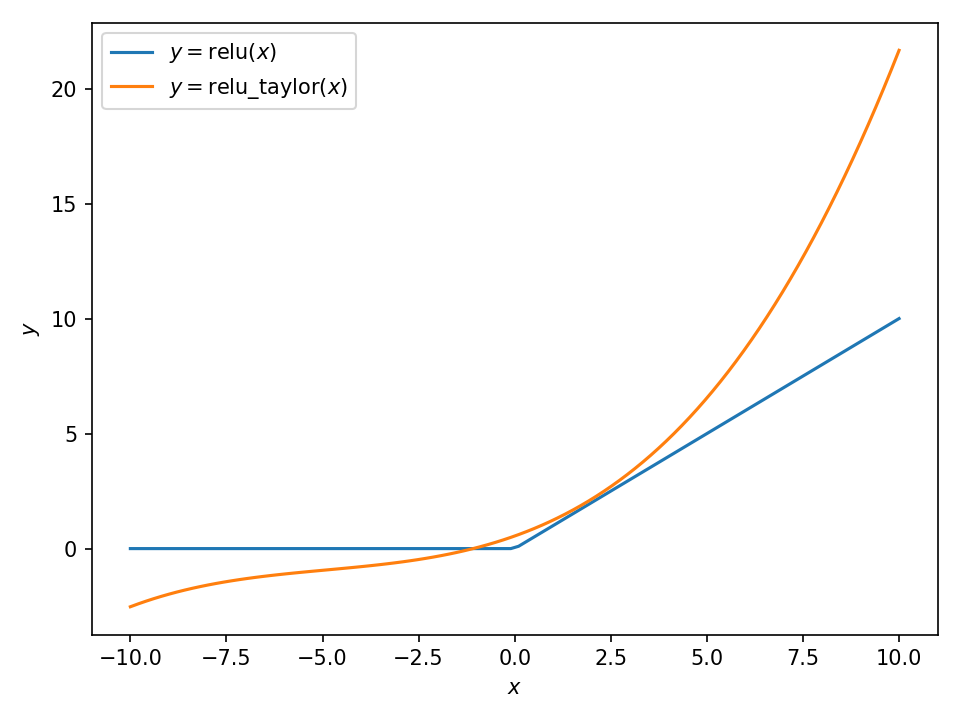
\includegraphics[width=0.8\linewidth]{figures/taylor-relu.png}
  \caption{Comparison of the Relu activation function vs. its Taylor expansion}
\end{figure}

\section{Notation and Acronyms}
\label{sec:gloss}
Symbols and acronyms are defined in the preamble, after loading the \texttt{glossaries} package, and used as follows.

In this chapter, we introduce the necessary background on the \gls{aes}.
We denote binary exclusive-or by \gls{xor}.

\label{sec:bib}
This is an example of how to specify and cite
a book \cite{AESbook},
a journal article \cite{bstjShannon49}.
\Gls{aes} is a block cipher defined by \textcite{AESbook}.
